\documentclass[aspectratio=169]{beamer}

\usepackage{mymacros}

\usepackage{graphicx}
  \graphicspath{{figures}}

\usepackage{subcaption}

\usetheme{firedrake}

\title{\texttt{pyop3} is coming}
\author{Connor Ward, David Ham, Jack Betteridge}
\date{16/09/2024}

\begin{document}

\frame{\titlepage}

\begin{frame}
  \begin{itemize}
    \item
      We have made a new package for \textbf{mesh stencil calculations}.
    \item
      It is called \pyop3.
    \item
      It will \textbf{soon replace \pyop2} in Firedrake.
    \item
      This presentation will focus on the impact this will have on you, Firedrake users and developers.
    \item
      And hopefully inspire some of you to give it a try.
  \end{itemize}
\end{frame}

\begin{frame}{Mesh stencil calculations}
  \vspace{-2em}
  \begin{center}
    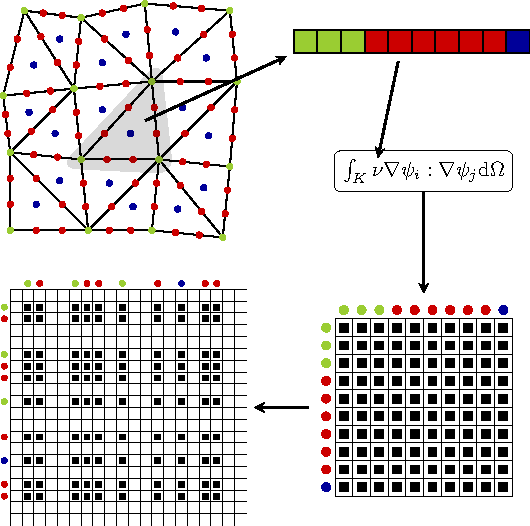
\includegraphics[scale=.9]{fem_assembly.pdf}
  \end{center}
\end{frame}

\begin{frame}{Introducing \pyop2: motivation}
  \begin{itemize}
    \item 
      Writing one assembly loop is easy, writing many is hard.
    \item
      Changing algorithms and architectures mean that we need to be able to make high-level changes to various aspects of the computation.
    \item
      We don't want to write these all by hand. Instead we want to automatically generate fast code.
  \end{itemize}
\end{frame}

\begin{frame}[fragile]{Introducing \pyop2}
  \pyop2 code:
  \begin{center}
    \begin{minted}[autogobble,linenos]{python}
      op2.par_loop(
        local_kernel,
        mesh.cell_set,
        dat(op2.READ, cell_node_map),
        mat(op2.INC, (cell_node_map, cell_node_map)),
      )
    \end{minted}
  \end{center}

  \vspace{1em}

  \begin{itemize}
    \item Generates, compiles, and executes C code.
    \item Automatically ensures parallel correctness.
    \item Much faster than a non-code-generated approach.
  \end{itemize}
\end{frame}

\begin{frame}{Why do we need something new?}
  \pyop2 is a wonderful tool, but...

  \begin{itemize}
    \item
      It was designed specifically for FEM.
    \item
      Some important classes of algorithm are not expressible or require non-composable `hacky' solutions.
  \end{itemize}
\end{frame}

\begin{frame}{Introducing \pyop3}
  \begin{itemize}
    \item A near-total rewrite of \pyop2.
    \item Still generates C code from a Python DSL.
    \item Has a much more flexible interface.
    \item Introduces a novel, flexible way of describing data layouts (later).
  \end{itemize}
\end{frame}

\begin{frame}{Introducing \pyop3}
  \vspace{-2em}
  \begin{center}
    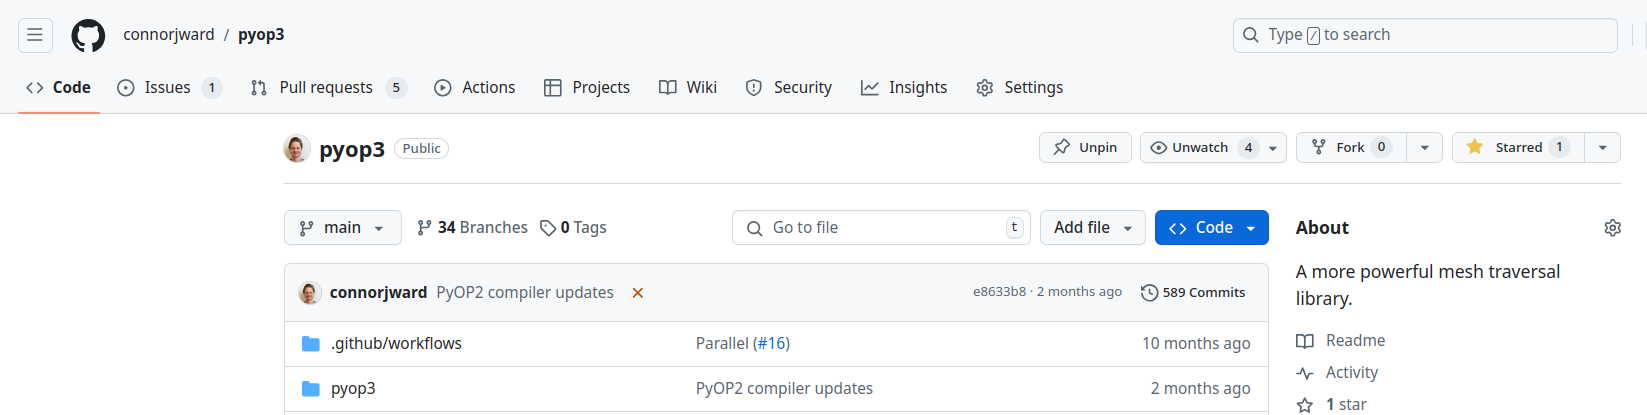
\includegraphics[width=\textwidth]{pyop3_github.png}
  \end{center}

  \begin{overprint}
    \onslide<1>\centering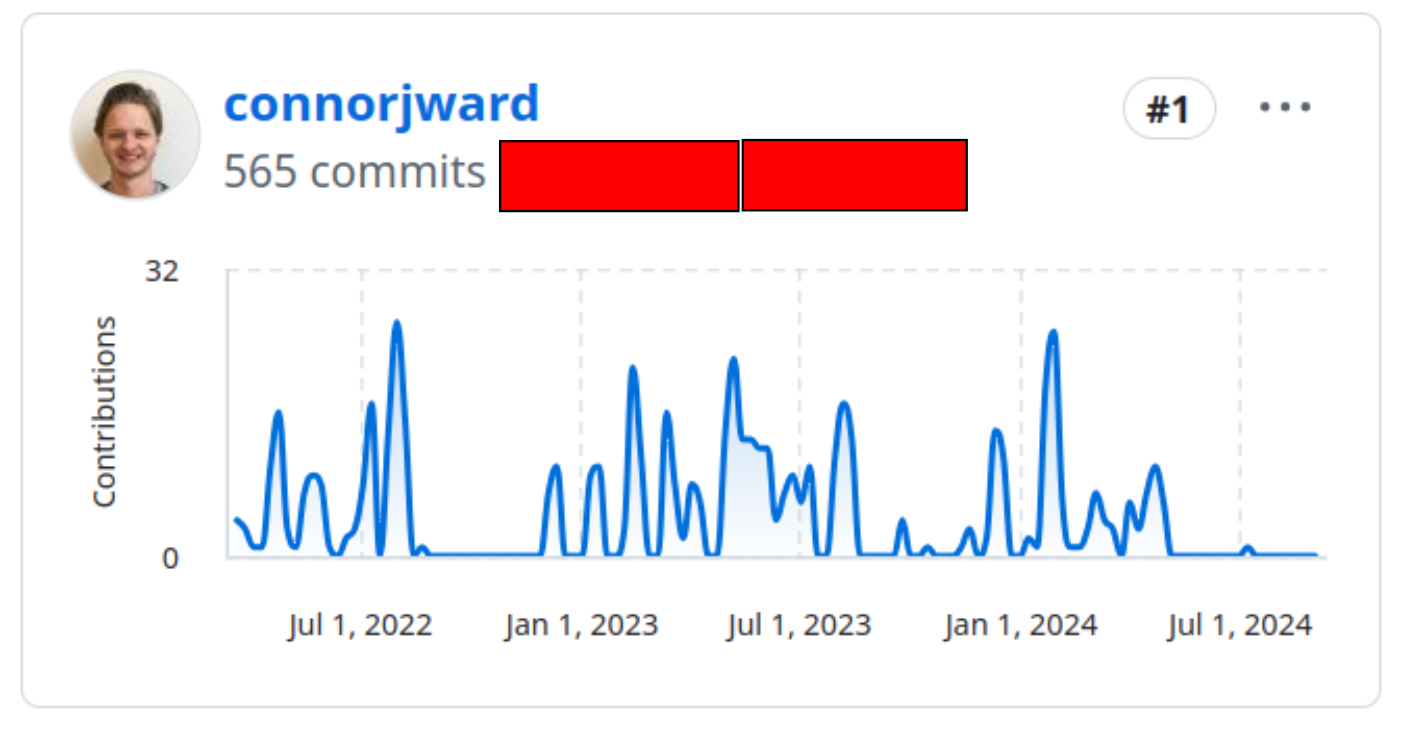
\includegraphics[width=.5\textwidth]{pyop3_github_stats_hidden.png}
    \onslide<2>\centering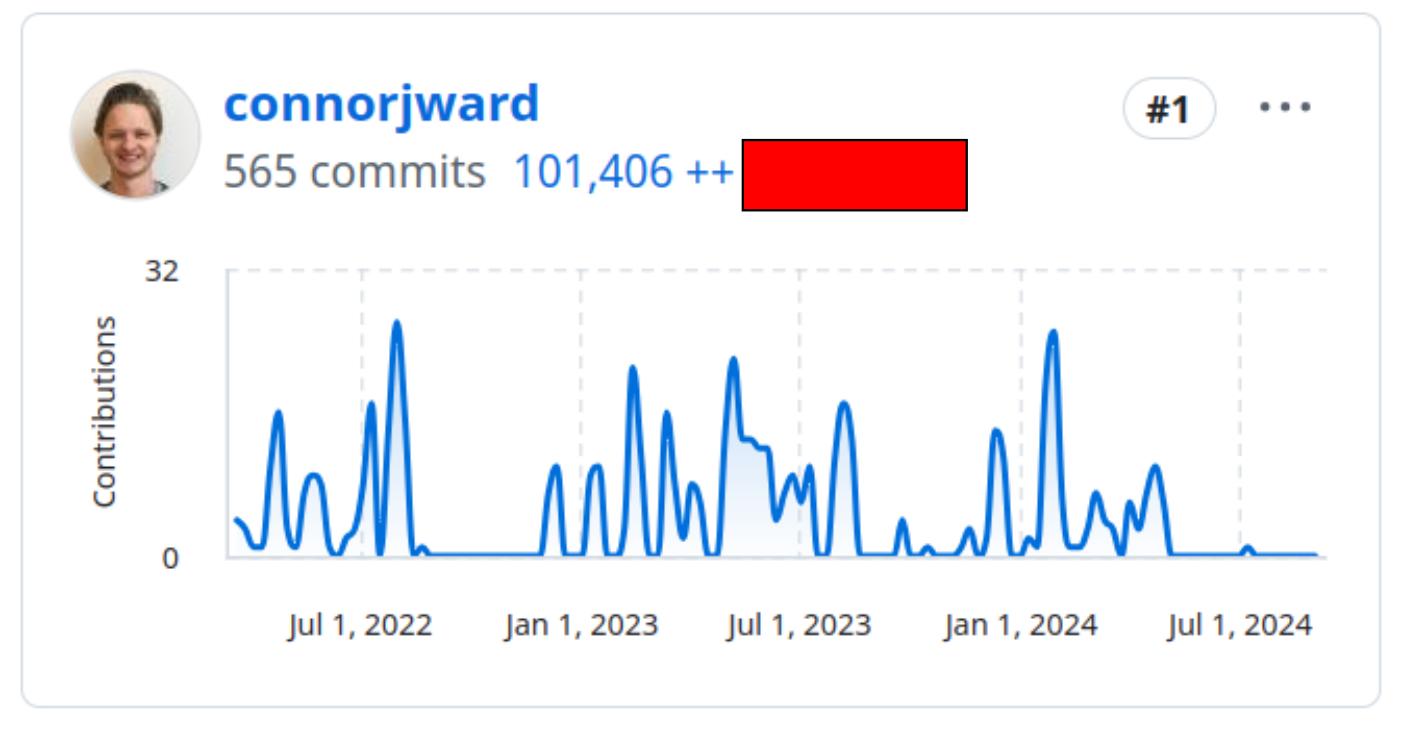
\includegraphics[width=.5\textwidth]{pyop3_github_stats_partial.png}
    \onslide<3>\centering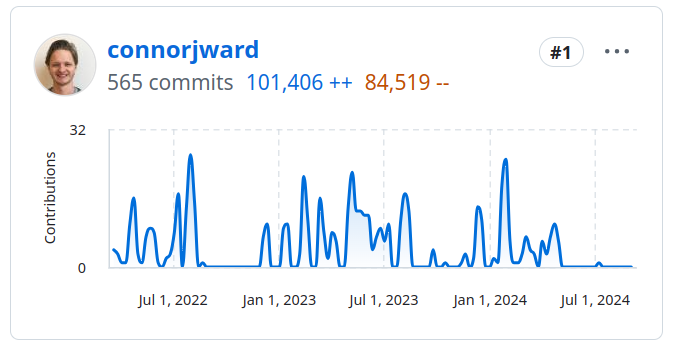
\includegraphics[width=.5\textwidth]{pyop3_github_stats_full.png}
  \end{overprint}
\end{frame}

\begin{frame}[fragile]{An example: vertex-based slope limiter}
  \vspace{-2em}
  \begin{columns}
    \begin{column}{0.5\textwidth}
      \begin{center}
        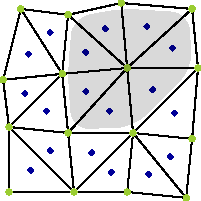
\includegraphics[width=.8\textwidth]{slope_limiter.pdf}
      \end{center}
    \end{column}
    \begin{column}{0.5\textwidth}
      \begin{minted}[autogobble,linenos,fontsize=\footnotesize]{python}
        mesh = UnitSquareMesh(...)
        V_cg = FunctionSpace(mesh, "CG", 1)
        V_dg = FunctionSpace(mesh, "DG", 0)
        cg = Function(V_cg)
        dg = Function(V_dg)

        loop = op3.loop(
          v := mesh.vertices.index(),
          op3.loop(
            c := mesh.star(v, k=2).index(),
            max_kernel(dg.dat[c], cg.dat[v]),
          ),
        )
        loop()
      \end{minted}
    \end{column}
  \end{columns}
\end{frame}

\begin{frame}[fragile]{An example: vertex-based slope limiter}
  \vspace{-1em}
  \inputminted[fontsize=\footnotesize,linenos]{c}{c_code_tidy.c}
\end{frame}

\begin{frame}{Flexibly describing data layouts}
  Data layouts are \textbf{trees}, instead of N-dimensional arrays.

  \begin{figure}
    \centering
    \begin{subfigure}{.49\textwidth}
      \centering
      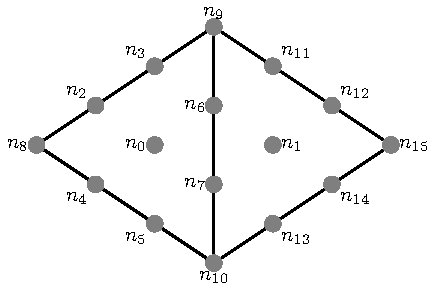
\includegraphics[width=.8\textwidth]{two_cell_mesh_lagrange_nodal.pdf}
    \end{subfigure}
    \begin{subfigure}{.49\textwidth}
      \centering
      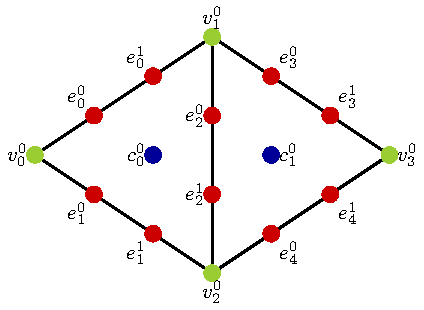
\includegraphics[width=.8\textwidth]{two_cell_mesh_lagrange.pdf}
    \end{subfigure}

    \begin{subfigure}{.49\textwidth}
      \centering
      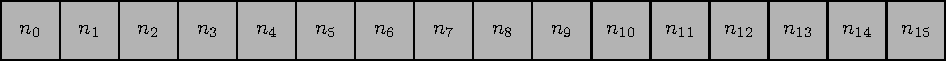
\includegraphics[width=\textwidth]{two_cell_mesh_lagrange_data_layout_flat_nodal.pdf}
    \end{subfigure}
    \begin{subfigure}{.49\textwidth}
      \centering
      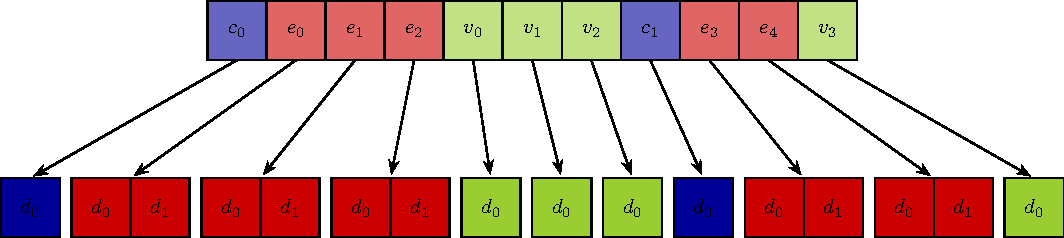
\includegraphics[width=\textwidth]{two_cell_mesh_lagrange_data_layout_nested.pdf}
    \end{subfigure}
  \end{figure}
\end{frame}

\begin{frame}{Flexible data layouts}
  \begin{itemize}
    \item
      \pyop3 can freely swap around tree nodes (axes) to give different, equivalent, data layouts.
    \item
      It is very similar to AoS/SoA optimisations.
  \end{itemize}

  \begin{center}
    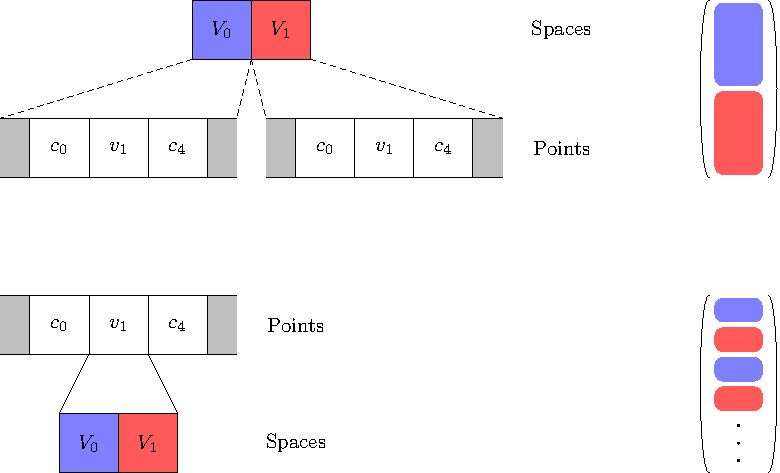
\includegraphics[width=.6\textwidth]{transform.pdf}
  \end{center}
\end{frame}

\begin{frame}{Impact on Firedrake}
  \begin{itemize}
    \item
      Hopefully extremely minimal. The top-level API is unchanged.
    \item
      If you are frequently interacting directly with the arrays (i.e. \pycode{function.dat.data}) then you \emph{may} notice changes.
    \item
      Obviously any \pyop2 code will need porting.
    \item
      Code performance should be unchanged.
  \end{itemize}
\end{frame}

\begin{frame}{Additional benefits}
  \begin{itemize}
    \item
      `Easy' to implement new preconditioners: SLATE (hybridisation) and PatchPC (additive Schwartz) are expressible by \pyop3.
    \item
      Can generate the transformation code necessary for arbitrary mesh entity orientations.
    \item Support for monolithic assembly of matrices containing Real blocks (incidental).
  \end{itemize}

  \vspace{1em}

  More speculative:

  \begin{itemize}
    \item Structured meshes
    \item $hp$-adaptivity
    \item Low-level compiler optimisations (e.g. loop fusion)
  \end{itemize}
\end{frame}


\begin{frame}{Farewell extruded mesh}
  \begin{columns}
    \begin{column}{.5\textwidth}
      \begin{center}
        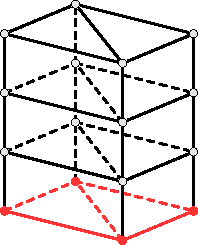
\includegraphics[width=.6\textwidth]{extruded.pdf}
      \end{center}
    \end{column}
    \begin{column}{.5\textwidth}
      Fast for 2 reasons:
      \begin{enumerate}
        \item Regular data layout
        \item Smaller indirection maps:
          \begin{equation*}
            \textnormal{loc} = \pycode{map0[?$i_{\textnormal{base}}$?]} + i_{\textnormal{column}} \times \textnormal{offset}
          \end{equation*}
      \end{enumerate}
      \pause

      \begin{itemize}
        \item
          It turns out that (2) \emph{is not very important}.

        \item
          An extruded mesh will just be a PETSc DMPlex.
          Lots of code can be simplified.
      \end{itemize}
    \end{column}
  \end{columns}
\end{frame}

\begin{frame}{Summary}
  \begin{itemize}
    \item
      \pyop3 will replace \pyop2 soon.
    \item
      It should enable a variety of new numerical methods.
    \item
      User-facing changes should be limited.
  \end{itemize}

  \vspace{1em}

  \begin{itemize}
    \item
      We are currently seeking funding to extend \pyop3 to support assembly on GPUs.
    \item
      Please consider giving it a try! (not just yet)
  \end{itemize}
\end{frame}

% \begin{frame}{Roadmap}
%   \pause
%   \vspace{-3em}
%   
\includegraphics[width=\textwidth]{shark.png}
% \end{frame}
%
% \begin{frame}{Roadmap (continued)}
%   \begin{itemize}
%     \item
%       \pyop3 should be merged within the next 6 months.
%     \item
%       It will be in a usable state well before then.
%     \item
%       Hopefully then we will have funding for me to get it working on GPUs.
%   \end{itemize}
% \end{frame}

\end{document}
